\documentclass{standalone}
\usepackage{tikz}
\usetikzlibrary{shapes, arrows.meta} % For node shapes and arrow styles
\begin{document}

Exercice 3

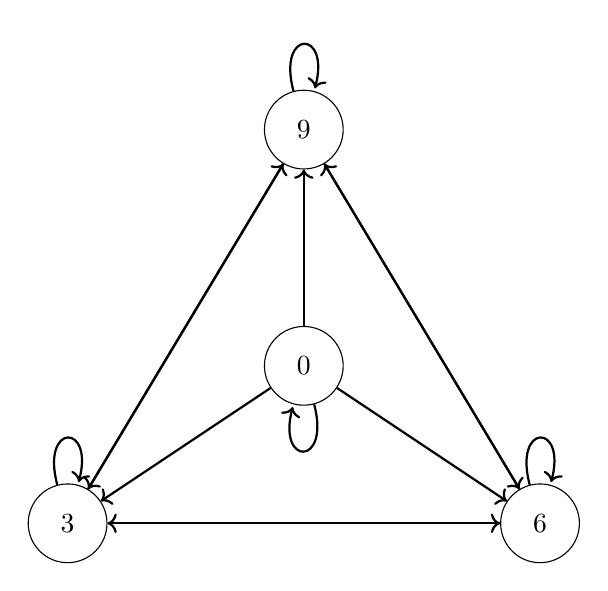
\begin{tikzpicture}

    \node[circle, draw, minimum size=1cm] (n0) at (0, 1) {0};
    \node[circle, draw, minimum size=1cm] (n3) at (-3, -1) {3};
    \node[circle, draw, minimum size=1cm] (n6) at (3, -1) {6};
    \node[circle, draw, minimum size=1cm] (n9) at (0, 4) {9}; 
    % Directed edges
    \draw[->, thick] (n0) edge[loop below] (n0); % Self-loop at node 0
    \draw[->, thick] (n3) edge[loop above] (n3); % Self-loop at node 3
    \draw[->, thick] (n6) edge[loop above] (n6); % Self-loop at node 6
    \draw[->, thick] (n9) edge[loop above] (n9); % Self-loop at node 9
    % Edges from 0 to others
    \draw[->, thick] (n0) -- (n3); % Edge from node 0 to node 3
    \draw[->, thick] (n0) -- (n6); % Edge from node 0 to node 6
    \draw[->, thick] (n0) -- (n9); % Edge from node 0 to node 9
    % Edges between 3, 6, and 9
    \draw[->, thick] (n3) -- (n6); % Edge from node 3 to node 6
    \draw[->, thick] (n6) -- (n3); % Edge from node 6 to node 3
    \draw[->, thick] (n3) -- (n9); % Edge from node 3 to node 9
    \draw[->, thick] (n9) -- (n3); % Edge from node 9 to node 3
    \draw[->, thick] (n6) -- (n9); % Edge from node 6 to node 9
    \draw[->, thick] (n9) -- (n6); % Edge from node 9 to node 6
\end{tikzpicture}

\begin{tikzpicture}
    \node[circle, draw, minimum size=1cm] (n1) at (0, 1) {1};
    \node[circle, draw, minimum size=1cm] (n4) at (-3, -1) {4};
    \node[circle, draw, minimum size=1cm] (n7) at (3, -1) {7};
    \node[circle, draw, minimum size=1cm] (n10) at (0, 4) {10}; 
    % Directed edges
    \draw[->, thick] (n1) edge[loop below] (n1); % Self-loop at node 0
    \draw[->, thick] (n3) edge[loop above] (n4); % Self-loop at node 3
    \draw[->, thick] (n6) edge[loop above] (n7); % Self-loop at node 6
    \draw[->, thick] (n9) edge[loop above] (n10); % Self-loop at node 9
    % Edges from 0 to others
    \draw[->, thick] (n0) -- (n3); % Edge from node 0 to node 3
    \draw[->, thick] (n0) -- (n6); % Edge from node 0 to node 6
    \draw[->, thick] (n0) -- (n9); % Edge from node 0 to node 9
    % Edges between 3, 6, and 9
    \draw[->, thick] (n3) -- (n6); % Edge from node 3 to node 6
    \draw[->, thick] (n6) -- (n3); % Edge from node 6 to node 3
    \draw[->, thick] (n3) -- (n9); % Edge from node 3 to node 9
    \draw[->, thick] (n9) -- (n3); % Edge from node 9 to node 3
    \draw[->, thick] (n6) -- (n9); % Edge from node 6 to node 9
    \draw[->, thick] (n9) -- (n6); % Edge from node 9 to node 6
\end{tikzpicture}

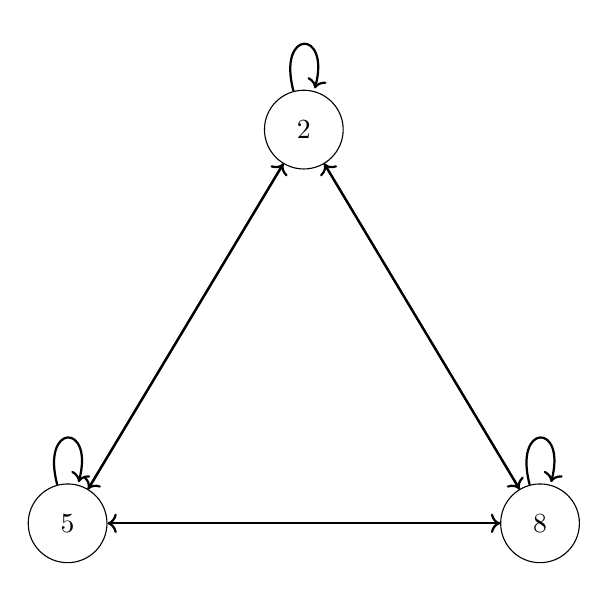
\begin{tikzpicture}
    \node[circle, draw, minimum size=1cm] (n5) at (-3, -1) {5};
    \node[circle, draw, minimum size=1cm] (n8) at (3, -1) {8};
    \node[circle, draw, minimum size=1cm] (n2) at (0, 4) {2}; 

    \draw[->, thick] (n5) edge[loop above] (n5); % Self-loop at node 3
    \draw[->, thick] (n8) edge[loop above] (n7); % Self-loop at node 6
    \draw[->, thick] (n2) edge[loop above] (n10); % Self-loop at node 9
    % Edges from 0 to others
    \draw[->, thick] (n2) -- (n5); % Edge from node 0 to node 3
    \draw[->, thick] (n2) -- (n8); % Edge from node 0 to node 6
    \draw[->, thick] (n5) -- (n2); % Edge from node 0 to node 9
    \draw[->, thick] (n5) -- (n8);
    \draw[->, thick] (n8) -- (n2); % Edge from node 0 to node 9
    \draw[->, thick] (n8) -- (n5);

\end{tikzpicture}

b)

\end{document}
